%\documentclass[11pt,a4paper,twoside]{book}
\documentclass[11pt,a4paper,oneside]{book}
 %\documentclass[oneside]{book}
% Misc
\usepackage[nottoc]{tocbibind} % Bibliography in toc
\usepackage{makeidx} \usepackage{graphicx} \usepackage{color}
\usepackage{parskip} \usepackage{natbib}
\definecolor{hhblue}{RGB}{0,73,133}

% Fancy headers
\usepackage{fancyhdr} \lhead{\slshape \nouppercase{\rightmark}}
\rhead{\slshape \nouppercase{\leftmark}}

% AMS Packages
\usepackage[intlimits]{amsmath} \usepackage{amscd}
\usepackage{amsxtra} \usepackage{amssymb}

% Hyperlinks
\usepackage{hyperref}
\hypersetup{colorlinks=true,linkcolor=hhblue,citecolor=hhblue,urlcolor=hhblue}

% Language
\usepackage[T1]{fontenc} \usepackage[swedish]{babel}
\usepackage[utf8]{inputenc}

%\iffalse
\usepackage{titlesec}
\titleformat{\chapter}[display]
  {\normalfont\huge\bfseries}{}{0pt}{\Huge}
  %{\normalfont\huge\bfseries}{}{0pt}{\Huge}
  {\normalfont\huge\bfseries\color{hhblue}}
\titlespacing*{\chapter}
  {0pt}{10pt}{30pt} % changed
%\fi
% Font
\usepackage[sc]{mathpazo} \usepackage{palatino}

% Page setup
\unitlength=1mm \oddsidemargin 0.0cm \evensidemargin 0.0cm \topskip
0.0cm \topmargin -0.5cm
% \headheight 0.0cm \headsep 0.0cm
\textheight 24.0cm \textwidth 16cm
\let\cleardoublepage\clearpage
\setcitestyle{super}


\usepackage{float}
\restylefloat{table}

\setlength{\arraycolsep}{1.4pt}


\begin{document}
\pagestyle{empty}

\frontmatter

% Framsida---------------------------------------------------------------------
\begin{titlepage}
  \begin{center}
  \end{center}
  \vspace{3cm}
  \begin{center}
    \hrule \vspace{0.5cm}
    {\Huge \bfseries \sffamily \color{hhblue} Projektplan(Raviolimaskin)}\\
   % \vspace{0.5cm} {\Large\emph{Kanske behövs någon undertext också}}
    \vspace{0.8cm} \hrule \vspace{2cm} {\Large{Reshad Ahmadi , Maryam Bayat}}\\
   %\hspace{1.5cm}
    %{\Large{Kalle Anka}}\\
    \vspace{2cm}
    \today\\
    \vspace{3cm}
    Examensarbete (Raviolimaskin)\\
    \vspace{1.5cm}
    Handledare: Kenneth Nilsson\\
   %\hspace{1.5cm}
    %{Tommy Salomonsson}\\ 
    \vspace{0.5cm} Examinator: Björn Åstrand \vfill
    
\includegraphics[width=4cm]{images/hh_logo.jpg}\\
    HÖGSKOLAN I HALMSTAD\\
    Sektionen för Informationsvetenskap, \\
    Data- och Elektroteknik
  \end{center}
\end{titlepage}

% Sammanfattning----------------------------------------------------------------
%\chapter{Sammanfattning}
%\chapter{Abstract}
%Here is the nice abstract written in english.
% Förord-----------------------------------------------------------------------
%\chapter{Förord}
%\pagestyle{fancy}
% Innehållsförteckning---------------------------------------------------------
%\tableofcontents
%\mainmatter
%Here is the nice abstract written in english.
% Förord-----------------------------------------------------------------------
%\chapter{Förord}
%\pagestyle{fancy}


% Innehållsförteckning---------------------------------------------------------
\tableofcontents
\mainmatter

\chapter{Introduktion}
Detta projekt ämnat till att utveckla en Raviolimaskin. Ravioli är en traditionell italiensk maträtt bestående av runda eller kvadratiska pastadeg med fyllning~\cite{engproc}. Fyllningen kan bestå av till exempel köttfärs, skinka och ost. Raviolin serveras ofta i en tomatsås eller köttfärssås. Vegetarisk ravioli kan exempelvis fyllas med purjolök eller spenat.

Att laga Ravioli hemma manuellt har varit jobbigt och tidskrävande. Det finns olika typer av Raviolimaskiner på marknaden just nu som hjälper med Raviolis ifyllnings process. 

Den enklaste typen av Raviolimaskin(Ravioliplatta) visas på figue ~\ref{ravioliplatta}. Den underlättar processen, men ifyllning av Raviolin görs manuellt som medför att det tar tid och använda det.

 
	\begin{figure}[h]
		\begin{center}
			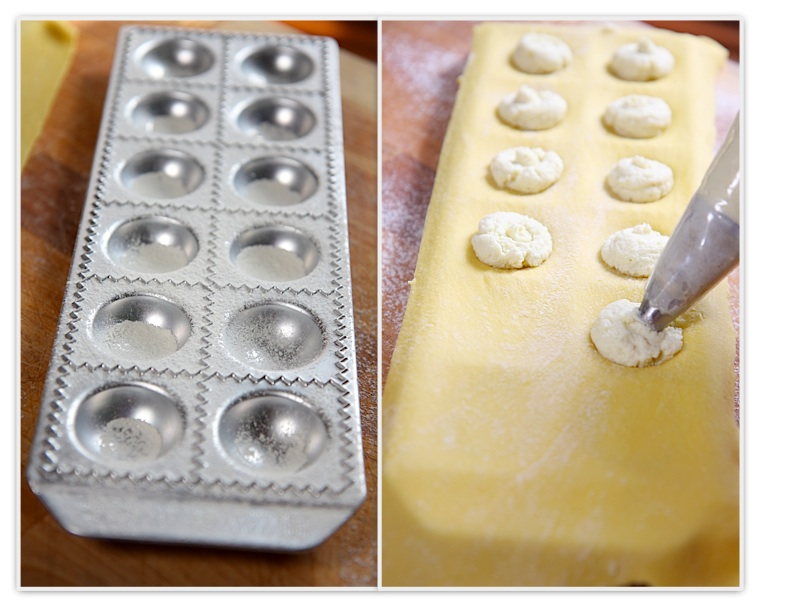
\includegraphics[scale=0.5]{images/raviolimoldwithfilling.jpg}
			\caption{Ravioliplatta för manuell fyllning av Ravioli}
			\label{ravioliplatta}	
		\end{center}
	\end{figure}
En annan typ av maskin som illustreras på figur~\ref{pastamaskin}, är väldigt stor och priset är högt som medför att de inte kan användas av hushåll.

Idén bakom detta projekt baseras på behovet av en Raviolimaskin hemma. Tanken är att utveckla en liten och relativ billig Raviolimaskin som kan vara användbar hemma.
 		\begin{figure}[h]
 			\begin{center}
 				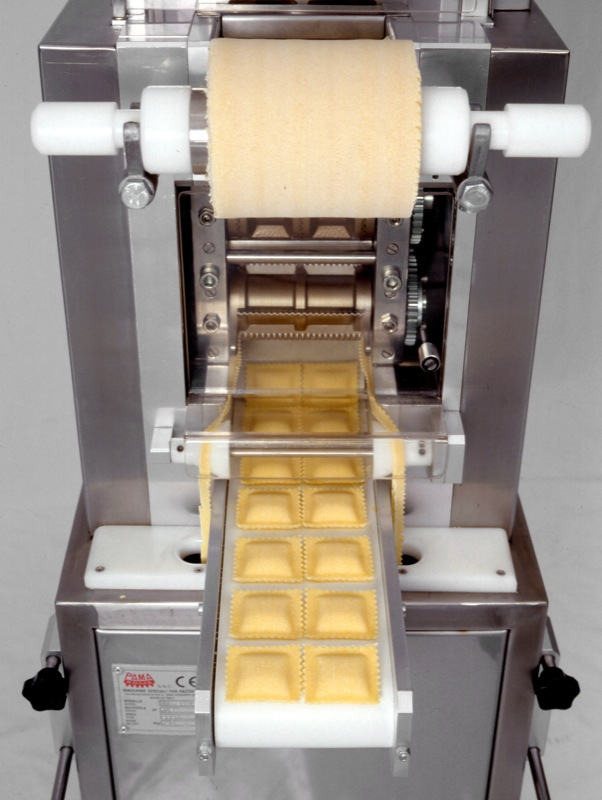
\includegraphics[scale=3]{images/pastamachine.jpg}
 				\caption{Industriell Pasta-/Raviolimaskin}
 				\label{pastamaskin}	
 			\end{center}
 		\end{figure} 

\section{Syfte och mål} % Goals
\\*

Detta projekts syfte är att utveckala en Ravioli maskin som (gör det mesta som en industeriell maskin gör men det ska vara)är rätt anpassad till hushåll i storleken, priset och användbarheten. Det är tänkt att användaren kan använda olika typer av ifyllnings material på maskinen.\\*

Maskinen är tänkt att göra det mesta av processen själv, genom att fylla Ravioli degar med ifyllnings material och stänger dem i slutet.




\section{Begränsningar} % Constraints

Eftersom tiden är låst till en deadline som inte kan flyttas , och personalresurer är begränsande 
vi kommer inte ha maskinen i metall. Vi avgränsar oss till att ha en plastmodell på slutet av projektet. För att det är rätt mycket material som måste skrivas ut på 3D-skrivare , vilket innebär att det krävs mycket tid åt varje del.

<<<<<<< HEAD
=======
En avgränsning ska vara att alla maskinens delar kommer att konstrueras med använndning av 3D-skrivare och plast som material. 
\iffalse
Eftersom existerande verktyg som används är den enda stora begränsningen den tid det tar att genomföra 
projektet. Tiden är låst till en deadline som inte kan flyttas, och personalresurser är begränsade. 
Följaktligen är kvaliteten den enda variabel som kan ändras om projektet löper risk att inte bli klar 
på utsatt tid.
\fi
>>>>>>> d29afcd0fbd569f0d8a96f491e801229ac5807ba


%-----------------------------------------------------------
\newpage
\chapter{Metod}
\section{Kunskapsläge}
Raviolimaskinen ska bestå av några mekaniska delar. För att designa maskinens delar ska CAD-tekniker användas. Att använda CAD-tekniker hjälper att rita maskinens olika delar och se resultatet innan man börjar konstruera dem fysiskt. Genom att designa med ett CAD-program, har man också möjligheten att analysera hållfasthet av maskinens delar genom att påverka virtuell kraft på dem. 


En mekanisk del av maskinen är en degform. Figuren ~\ref{degfrom} visar en dagform som används för att knyta Raviolidegen manuellt genom att trycka på formens sidor. För detta projekt har planerats att en eller två motorer ska trycka degformens sidor. Olika tekniker för att överföra motorers rörelseenergi till Raviolimaskinens degform ska undersökas. 

\begin{figure}[h]
	\begin{center}
		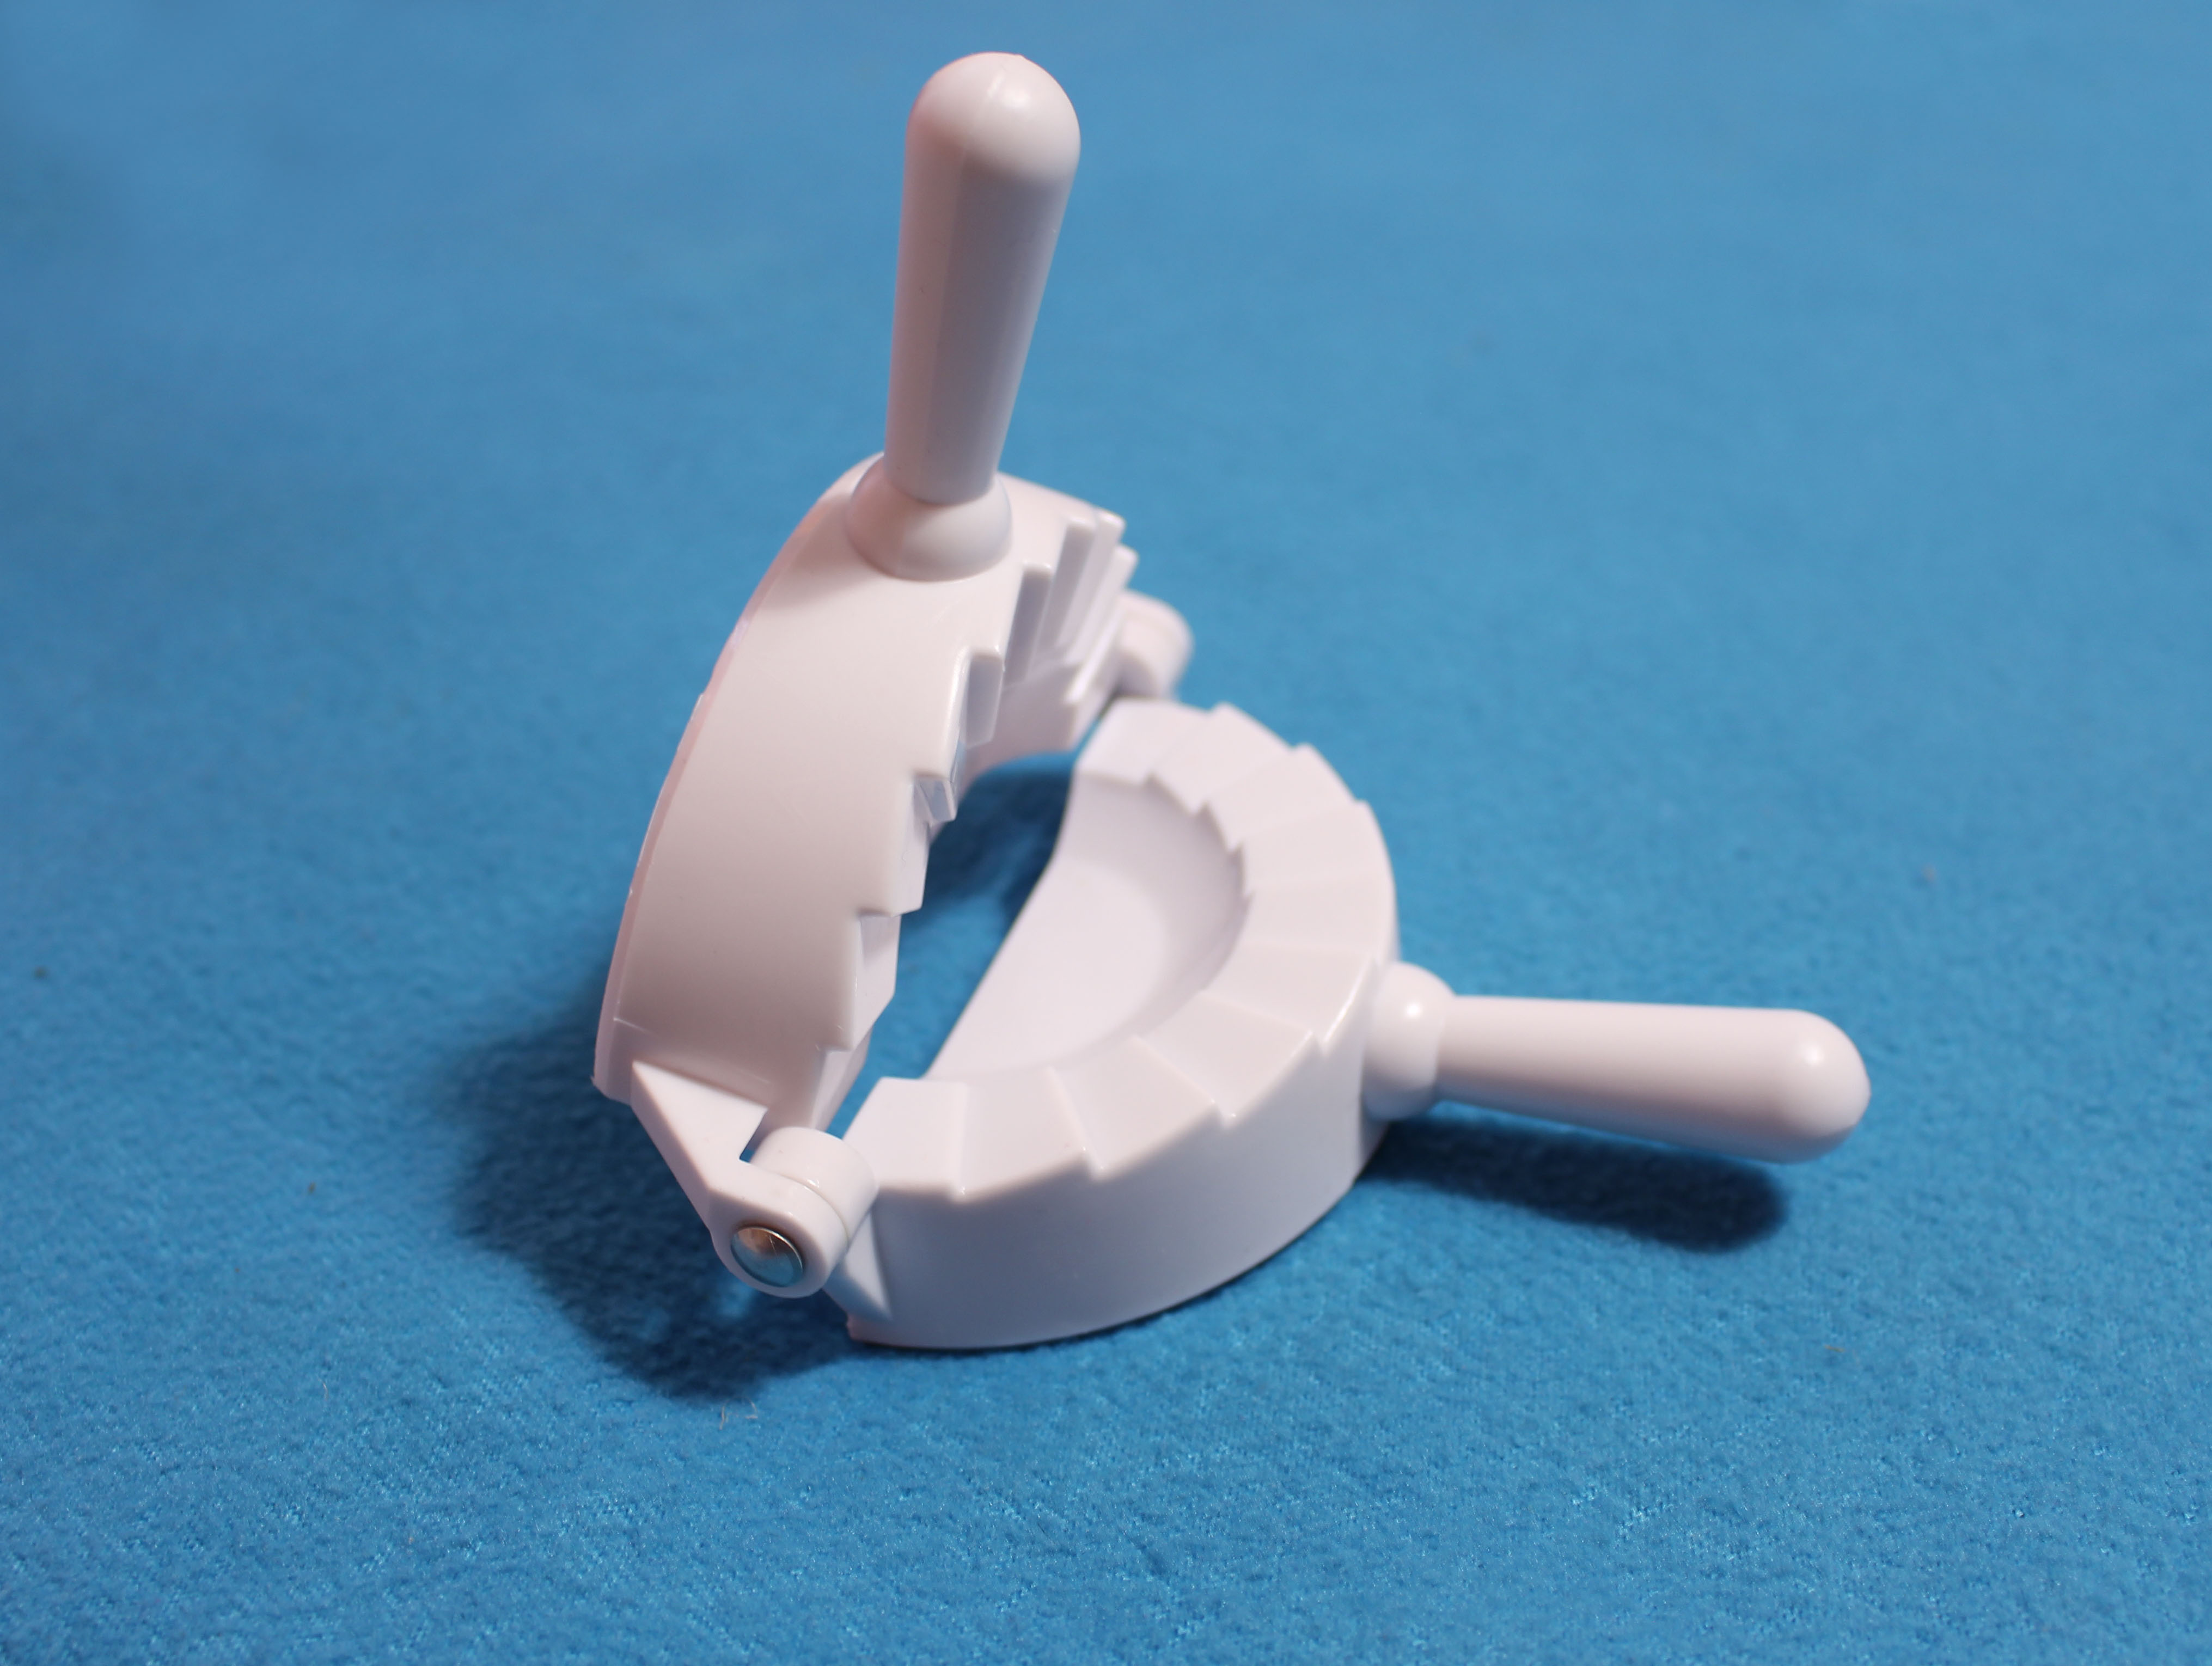
\includegraphics[scale=0.08] {images/degform.jpg}
		\caption{Degform för manuell ifyllning}
		\label{degfrom}	
	\end{center}
\end{figure}

En annan teknik som ska användas på detta projekt är regleringsteknik. Reglering kommer vara användbar när det gäller att reglera t.ex. den strömmen som går till elektroniska komponenter. Regleringsteknik kan också användas för eventuella systemidentifiering. 

Mikrokontrollern som ska användas för detta projekt är en Arduino Due. Programmeringsspråket ska vara C, men det är tänkt att använda Arduino IDE i fall man inte hinner programmera med C.






\section{Hur uppgifterna specifieras}
Uppgifterna specificerar genom att dela upp projektet i tre stora delar. Det första delen är mekanik som består av maskinens formgivning och analys av alla krafter som kommer påverkas på varje del. Kravet på mekaniken specificerar genom att varje del av maskinen ska orka bära de krafter som kommer påverka det.

Vidare ska finnas elektronikdel som består av en krets för att strömförsörja motorer och några eventuella sensorer. Krav på elektroniken kan specificera genom att alla komponenter(motorer och eventuella sensorer) får tillräcklig ström för att fungera rätt. Det är också tänkt att utveckla strömregulator som ska reglera strömmen som går till de elektroniska komponenter. 

Programmeringsdel av projektet tar hand om timingen på ett sätt att olika komponenter fungerar rätt och i rätt tid. Programmerings uppgifter omfattas att läsa av sensorers värde och driva motorer. 


\section{Metodbeskrivning}
Raviolimaskinens delar kommer konstrueras med hjälp av en 3D-skrivare. Detta mest för att det blir mycket lättare att skapa vissa delar som är svårt om man vill anlägga med metal. Det blir också billigare att printa delar med plast än bygga dem med t.ex. stål. Resursbehovet för att printa alla de delar är självklart tillgång till en 3D-skrivare, 4 dagar i vecka för en månad för att hinna med allt.\\

Projektets elektronik kommer utvecklas med användning av några elektroniska komponenter. En prototyp av kretsen ska byggas och användas under projektet. Ett kretskort kommer tillverkas när prototypen har fungerad som det ska. Resursbehovet för elektroniken utöver komponenterna ska möjligen vara tillgång till elverkstad för att kunna tillverka ett kortet.\\

Eftersom det är en egen ide, är det tänkt att använda skolan resurser liksom elverkstad eller 3D-skrivare. Nodvändiga Komponenter kommer liksom ABS-filament till 3D-printern eller elektronikska komponenter ska skaffas av projektets deltagare.




\section{Analys av resultat}
Projektet kan delas i Mekanik, elektronik och programmering. Mekanik testen genomförs på olika delar för att testa om de verkligen orkar bära de krafter som kommer påverka dem. Det finns mätutrustning liksom dynamometer för att mäta den kraften som en del måste kunna tåla. Man kan för testskul påverka lika mycket kraft på samma del för att kontrollera om den verkligen lyckas tåla den kraften.

Elektroniken kan analyseras genom att alla komponenter får den strömmen som är bestämt för dem. T.ex. om en motor skulle har fått 250 mA, kan man kontrollera att den försörjas med den bestämda strömmen under olika testfall och olika last på den.

För programmeringsdel kan testprogram skrivas som testar olika funktioner. Ett exempel för test av koden kan vara att kontrollera avläsning av en specifik sensor under en viss period och kontrollera resultatet. Mer specifik testfall för olika delar av Raniolinaskinen kommer speciferas när man har fått en tydligre bild av maskinen och dess olika delar.
\newpage



%\begin{itemize}
% \item Krav nr 1: Bygga en reglercentral som ska ersätta innedelen.
 %\item Krav nr 2: Reglercentralen ska kommunicera med utedelen enbart med RS-485 via kontakter F1 och F2.
% \item Krav nr 3: Reglercentralen ska hantera två insignaler. En analog signal mellan 0 till 10 volt och en digital signal.
% \item Krav nr 4: Reglercentralen ska översätta kompressorns frekvens så att tex 1 volt analog insignal motsvarar 10\% av kompressorn kapacitet, 2 volt 20 \% osv.
% \item Krav nr 5: Värme eller kylläge på utedelen ska väljas med den digitala insignalen till centralen.\\*
%\end{itemize}

\backmatter
% Referenser--------------------------------------------------------------------
\begin{thebibliography}{9}
\bibitem{engproc}
\href{http://www.wisegeek.com/what-is-ravioli.htm}{http://www.wisegeek.com/what-is-ravioli.htm}, engproc
\bibitem{max_485}
\href{https://www1.elfa.se/data1/wwwroot/assets/datasheets/jxMAX481E-491E_e.pdf}{MAX485}, Elfa
\bibitem{OSI}
\href{http://www.rejas.se/fritis/datorkommunikation/chap_protokoll.html}{OSI}, Rejas
\bibitem{Duplex}
\href{ http://en.wikipedia.org/wiki/Duplex_(telecommunications)}{Duplex}, Wikipedia
\bibitem{arduino}
\href{http://arduino.cc/en/Main/arduinoBoardDue}{Arduino due}, Arduino
\bibitem{RS och point-point mm}
\href{http://www.youtube.com/watch?v=2DQdEHvnqvI}{RS485}, Youtube
\bibitem{Om RS}
\href{http://www.ti.com/lit/an/slla070d/slla070d.pdf}{RS485}, Youtube
\bibitem{OSI modell}
\href{http://support.microsoft.com/kb/103884 }{RS485}, Youtube
\bibitem{CRC}
\href{http://en.wikipedia.org/wiki/Cyclic_redundancy_check }{CRC}, Wikipedia
\bibitem{Paritet}
\href{http://en.wikipedia.org/wiki/Parity_bit }{Paritet}, Wikipedia
\bibitem{Skillnader mellan RS korten}
\href{http://www.binarteknik.se/produkter/1201.phtml}{RS}, Wikipedia
\bibitem{RS485}
\href{http://en.wikipedia.org/wiki/RS-485}{RS485}, Wikipedia
\bibitem{Seriellt}
\href{http://www.rejas.se/fritis/datorkommunikation/chap_serpar.html}{Seriell}, Wikipedia
\iffalse
\bibitem{HALSALL} FRED HALSALL, {\it THRID EDITION DATA COMMUNICTIONS, COMPUTER NETWORKS AND OPEN SYSTEMS},Addsion wesley, Publishers (1994).
\bibitem{feynman} R. P. Feynman, {\it Phys. Rev.} {\bf 76}, 749 (1949); {\bf 76}, 769 (1949).
\fi
\end{thebibliography}

\end{document}
